%%%%%%%%%%%%%%%%%%%%%%%%%%%%%%%%%%%%%%%%%%%%%%%%%%%%%%%%%%%%%%%%%%%%%
% LaTeX Template: Project Titlepage Modified (v 0.1) by rcx
%
% Original Source: http://www.howtotex.com
% Date: February 2014
% 
% This is a title page template which be used for articles & reports.
% 
% This is the modified version of the original Latex template from
% aforementioned website.
% 
%%%%%%%%%%%%%%%%%%%%%%%%%%%%%%%%%%%%%%%%%%%%%%%%%%%%%%%%%%%%%%%%%%%%%%

\documentclass[12pt]{article}
\usepackage[a4paper]{geometry}
\usepackage[myheadings]{fullpage}
\usepackage{fancyhdr}
\usepackage{lastpage}
\usepackage{graphicx, wrapfig, subcaption, setspace, booktabs}
\usepackage[T1]{fontenc}
\usepackage[font=small, labelfont=bf]{caption}
\usepackage{fourier}
\usepackage[protrusion=true, expansion=true]{microtype}
\usepackage[english]{babel}
\usepackage{sectsty}
\usepackage{url, lipsum}
\usepackage{verbatim}

\newcommand{\HRule}[1]{\rule{\linewidth}{#1}}
\onehalfspacing
\setcounter{tocdepth}{5}
\setcounter{secnumdepth}{5}

%-------------------------------------------------------------------------------
% HEADER & FOOTER
%-------------------------------------------------------------------------------
\pagestyle{fancy}
\fancyhf{}
\setlength\headheight{15pt}
\fancyhead[L]{Kevin Klein}
%\fancyhead[R]{Anglia Ruskin University}
\fancyfoot[R]{Page \thepage\ of \pageref{LastPage}}
%-------------------------------------------------------------------------------
% TITLE PAGE
%-------------------------------------------------------------------------------

\begin{document}

\title{ \normalsize \textsc{Social Data Science project}
		\HRule{0.5pt} \\
		\LARGE How do internal and external reactions towards gains and losses of the S\&P 500 index differ?
		\HRule{2pt} \\ [0.5cm]
		\normalsize \today \vspace*{5\baselineskip}}

\date{}

\author{
		Kevin Klein \\
		github.com/kkleindev/SocialDataScience18}

\maketitle
%\tableofcontents
\newpage

%-------------------------------------------------------------------------------
% Section title formatting
\sectionfont{\scshape}
%-------------------------------------------------------------------------------

%-------------------------------------------------------------------------------
% BODY
%-------------------------------------------------------------------------------

\section{Motivation}
Humans are susceptible to a range of conscious biases\cite{evolution, kahneman}, which, many times, hinder objective assessments of situations. This project aims to identify skewed perspectives in the realm of investing. Understanding the difference in perception of other people's and oneself's success,
in other words obtaining a more realistic view is a precondition to consciously and actively counteracting biases such as the 'the grass is greener' effect. The hypothesis was to observe loss affection in one own's immediate inner reactions to information, called \emph{internal reactions}, and survivorship bias in the displayal of actions towards other people, called \emph{external reactions}. In order to do so, we assumed the number of related Google queries to be a proxy for the intensity of internal reactions and either the number of related reddit comments or their average sentiment intensity to be a proxy for external reactions.
\section{Data retrieval}
We refer to three datasets each comprising information on 254 weeks starting from February 17 2013. Each datapoint corresponds to a value assigned to one of the 254 weeks.

The financial data was provided by the Wall Street Journal \footnote{http://quotes.wsj.com/index/SPX/historical-prices} with daily opening and closing prices for the specified time range in USD.

The Google query quantification has been provided by Google Trends. In particular the \emph{S\&P 500} market index topic instead of a simple keyword search could be used. Unfortunately, for larger time ranges, results are restricted to be on a weekly basis. Moreover, this cannot be simply circumvented by merging data of many shorter time ranges, as the data represents locally normalized instead of global quantities. 

The reddit comment bodies stem from a publicly available dataset\footnote{https://files.pushshift.io/reddit/comments/} of all reddit comments from 2006 to 2017 . In particular, this dataset was accessed via Google Cloud's BigQuery platform \footnote{https://bigquery.cloud.google.com/dataset/fh-bigquery/reddit\_comments}. For a given week, all relevant comments were retrieved via a BigQuery library for python\footnote{https://cloud.google.com/bigquery/docs/reference/libraries\#client-libraries-install-python}. A comment was considered relevant if its body, turned lower case, contained the substring \emph{s\&p 500}. 

\section{Data processing}

For each date within the time range, the difference between closing and opening price was recorded and aggregated to a weekly mean, we will refer to this as \emph{change}. Weeks with strictly positive change are considered positive weeks, weeks with strictly negative change are considered negative weeks. Negative week changes were negated in order to represent positive values. When talking about absolute or amplitude changes, both positive and negative weeks are considered simultaneously.

Per week, the number of relevant reddit comments as well as their average sentiment have been recorded. The sentiment analysis is based on nltk's SentimentIntensityAnalyzer\footnote{http://www.nltk.org/api/nltk.sentiment.html}. The latter provided a compound polarity score per datapoint.

\section{Analysis}
Note that all p-values are double-sided as we are interested in whether some linear correlation exists in an absolute sense, independently of its sign. P-values have been determined via $10^5$ random permutations. 

\subsection{Internal reactions}
Correlations between change amplitude and the number of queries are below 0.2 for absolute changes, positive changes as well as negative changes, with p-values ranging from 0.006 to 0.084. Hence we have a reason to believe that only weak correlation exists. Still, let us investigate how regressions of positive and negative value changes look like in order to compare internal reactions to gains and losses.
\begin{figure}[!htb]
\minipage{0.32\textwidth}
  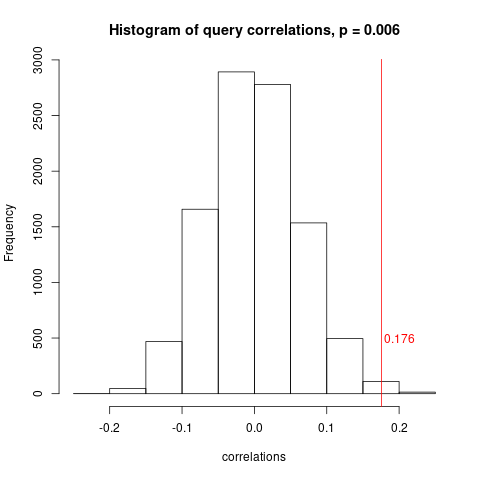
\includegraphics[width=\linewidth]{queryCorrelations.png}
  \caption{Correlations of value change amplitude and \#queries}\label{fig:trendCorrelation}
\endminipage\hfill
\minipage{0.32\textwidth}
  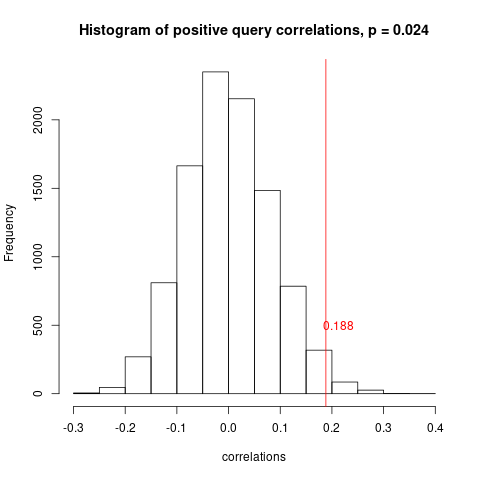
\includegraphics[width=\linewidth]{positiveQueryCorrelations.png}
  \caption{Correlations of positive value changes and \#queries}\label{fig:posTrendCorrelation}
\endminipage\hfill
\minipage{0.32\textwidth}%
  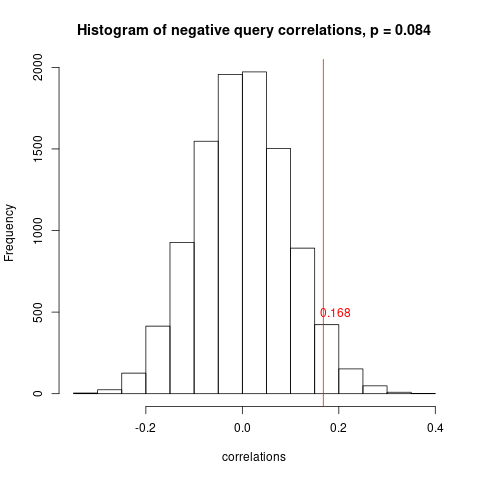
\includegraphics[width=\linewidth]{negativeQueryCorrelations.png}
  \caption{Correlations of negative value changes and \#queries}\label{fig:negTrendCorrelation}
\endminipage
\end{figure}

\begin{figure}[!]
\minipage{0.32\textwidth}
  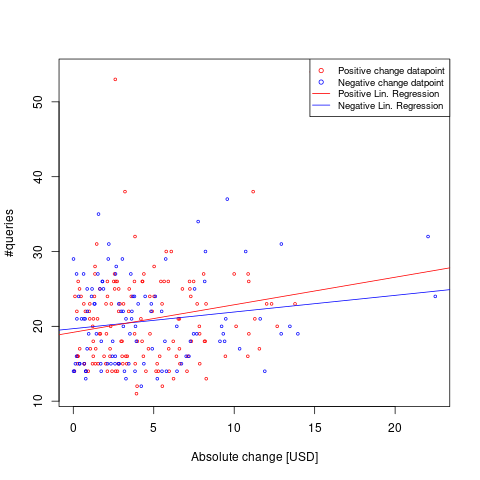
\includegraphics[width=\linewidth]{linearTrendRegressions.png}
  \caption{Linear fits for value changes to \#queries}\label{fig:linearTrendRegressions}
\endminipage\hfill
\minipage{0.32\textwidth}
  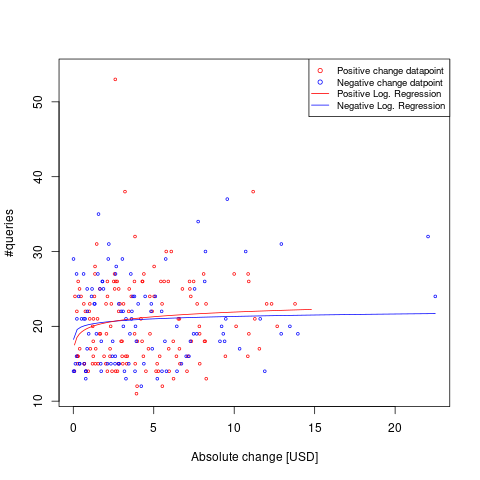
\includegraphics[width=\linewidth]{logTrendRegressions.png}
  \caption{Logarithmic fits for value changes to \#queries}\label{fig:logTrendRegressions}
\endminipage\hfill
\minipage{0.32\textwidth}
  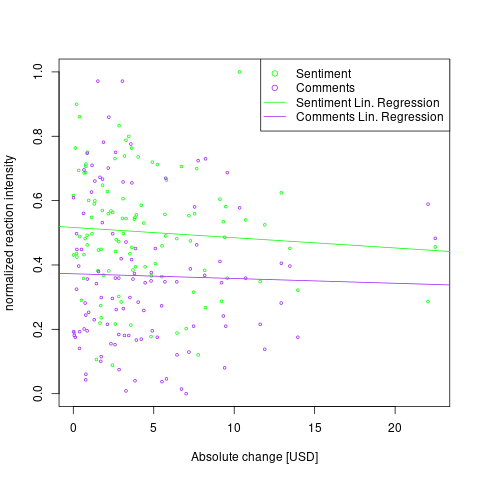
\includegraphics[width=\linewidth]{externalReactionsLosses.png}
  \caption{Linear fits for losses to sentiment insensity and \#comments}\label{fig:linExternalLosses}
\endminipage\hfill
\end{figure}

Both linear, figure \ref{fig:linearTrendRegressions}, and logistic, figure \ref{fig:logTrendRegressions}, regressions make it apparent that the number of queries grows with the amplitude of a value change. What cannot be clearly deduced is that people are distinctively loss-averse as neither fitted functions nor the points itself have remarkably higher query numbers for negative changes than for corresponding positive changes.

\subsection{External reactions}

We observe in table \ref{table:externalReactions} that both the number of comments as well as the sentiment intensity have very low observed correlation with high p-values. This holds for absolute changes, positive value changes as well as negative value changes. Remembering that correlation only allows us to make statements about linear dependencies, one might still consider to fit non-linear functions. Yet this is very unpromising as can be assessed by simply looking at a scatter plot in figure \ref{fig:linExternalLosses}. It becomes apparent that the data is simply too spread out. Hence there is no reason to believe that either the number of related reddit comments or their average sentiment intensity are useful indicators for external reactions.

\begin{table}[h!]
\centering
\begin{tabular}{|| c ||c c c c c c||} 
 \hline
 & Comm & PosComm & NegComm & Sent & PosSent & NegSent \\ [0.5ex] 
 \hline\hline
 cor & -0.048 & -0.067 & -0.028 & -0.076 & -0.082 & -0.072\\ 
 p & 0.454 & 0.423 & 0.778 & 0.223 & 0.336 & 0.463\\
 \hline
\end{tabular}
\caption{Correlation and p values of external reactions}
\label{table:externalReactions}
\end{table}

\section{Conclusion}

A comparison between internal and external reactions was not possible as the proxy data for external reactions was too close to random noise. For internal reactions, we found that there was some correlation between the value change of the index and the number of queries with legitimate p-values. Still, we were not able to observe a loss aversion effect in internal reactions.

\section{Critique}
Google Trend's restriction of only providing data per 5-day intervals is certainly a hurdle for determining reactions to a market index which can fluctuate heavily on a daily basis. This might simply dilute the effect of outliers. In particular, daily results would have been desirable. This also applies to the external reaction analysis, as the intention was to compare both. \\
In addition, it is very well imaginable that over such a long period, the different user numbers and behaviours of the referenced technologies might skew the numbers. Reddit is not to be considered in a 'steady state' but its user and comment counts, as well activity in specific subreddits fluctuate. Likewise, both the user behaviour of searching for a market index on Google as well as Google's counting methodology are prone to changes indepdent of user interest in market indices. 
%-------------------------------------------------------------------------------
% REFERENCES
%-------------------------------------------------------------------------------
\newpage
%\section*{References}
\begin{thebibliography}{9}

\bibitem{evolution}
Haselton, M. G.; Nettle, D. \& Andrews, P. W. (2005). The evolution of cognitive bias (PDF). In D. M. Buss (Ed.), The Handbook of Evolutionary Psychology: Hoboken, NJ, US: John Wiley \& Sons Inc. pp. 724–746.
 
 \bibitem{kahneman}
 Kahneman, D.; Tversky, A. (1972). "Subjective probability: A judgment of representativeness"
\end{thebibliography}

\end{document}

%-------------------------------------------------------------------------------
% SNIPPETS
%-------------------------------------------------------------------------------

%\begin{figure}[!ht]
%	\centering
%	\includegraphics[width=0.8\textwidth]{file_name}
%	\caption{}
%	\centering
%	\label{label:file_name}
%\end{figure}

%\begin{figure}[!ht]
%	\centering
%	\includegraphics[width=0.8\textwidth]{graph}
%	\caption{Blood pressure ranges and associated level of hypertension (American Heart Association, 2013).}
%	\centering
%	\label{label:graph}
%\end{figure}

%\begin{wrapfigure}{r}{0.30\textwidth}
%	\vspace{-40pt}
%	\begin{center}
%		\includegraphics[width=0.29\textwidth]{file_name}
%	\end{center}
%	\vspace{-20pt}
%	\caption{}
%	\label{label:file_name}
%\end{wrapfigure}

%\begin{wrapfigure}{r}{0.45\textwidth}
%	\begin{center}
%		\includegraphics[width=0.29\textwidth]{manometer}
%	\end{center}
%	\caption{Aneroid sphygmomanometer with stethoscope (Medicalexpo, 2012).}
%	\label{label:manometer}
%\end{wrapfigure}

%\begin{table}[!ht]\footnotesize
%	\centering
%	\begin{tabular}{cccccc}
%	\toprule
%	\multicolumn{2}{c} {Pearson's correlation test} & \multicolumn{4}{c} {Independent t-test} \\
%	\midrule	
%	\multicolumn{2}{c} {Gender} & \multicolumn{2}{c} {Activity level} & \multicolumn{2}{c} {Gender} \\
%	\midrule
%	Males & Females & 1st level & 6th level & Males & Females \\
%	\midrule
%	\multicolumn{2}{c} {BMI vs. SP} & \multicolumn{2}{c} {Systolic pressure} & \multicolumn{2}{c} {Systolic Pressure} \\
%	\multicolumn{2}{c} {BMI vs. DP} & \multicolumn{2}{c} {Diastolic pressure} & \multicolumn{2}{c} {Diastolic pressure} \\
%	\multicolumn{2}{c} {BMI vs. MAP} & \multicolumn{2}{c} {MAP} & \multicolumn{2}{c} {MAP} \\
%	\multicolumn{2}{c} {W:H ratio vs. SP} & \multicolumn{2}{c} {BMI} & \multicolumn{2}{c} {BMI} \\
%	\multicolumn{2}{c} {W:H ratio vs. DP} & \multicolumn{2}{c} {W:H ratio} & \multicolumn{2}{c} {W:H ratio} \\
%	\multicolumn{2}{c} {W:H ratio vs. MAP} & \multicolumn{2}{c} {\% Body fat} & \multicolumn{2}{c} {\% Body fat} \\
%	\multicolumn{2}{c} {} & \multicolumn{2}{c} {Height} & \multicolumn{2}{c} {Height} \\
%	\multicolumn{2}{c} {} & \multicolumn{2}{c} {Weight} & \multicolumn{2}{c} {Weight} \\
%	\multicolumn{2}{c} {} & \multicolumn{2}{c} {Heart rate} & \multicolumn{2}{c} {Heart rate} \\
%	\bottomrule
%	\end{tabular}
%	\caption{Parameters that were analysed and related statistical test performed for current study. BMI - body mass index; SP - systolic pressure; DP - diastolic pressure; MAP - mean arterial pressure; W:H ratio - waist to hip ratio.}
%	\label{label:tests}
%\end{table}